\section{CONCEPTOS GENERALES}

\subsection{Machine Learning}
Conocemos como Machine Learning a la rama de la computación que estudia el diseño de algoritmos que son capaces de aprender. Este tipo de algoritmos son utilizados en la actualidad para muchas aplicaciones, por ejemplo para recomendaciones de películas o para ranquear sitios web en base a una consulta.


\subsection{Algoritmo y Modelo}

Se parte de un algoritmo de Machine Learning y se desea obtener lo que conocemos como modelo, aquel que se adapte mejor a nuestro set de datos. El algoritmo es el enfoque general que se toma. El modelo es lo que se obtiene cuando se ejecuta el algoritmo sobre el set datos de entrenamiento y lo que se usa para hacer predicciones sobre nuevos datos. Se puede generar un nuevo modelo con el mismo algoritmo pero con datos diferentes, o un modelo diferente de los mismos datos con un algoritmo diferente. 
Cada modelo tiene un conjunto de parámetros e hiper-parámetros que necesita para funcionar. Los parámetros los descubre el algoritmo a partir de los datos, los hiper-parámetros, en cambio, son datos que debemos pasarle al algoritmo para funcionar\footnote{Apunte del curso, 11.1
Evaluación de Algoritmos de ML}. Por lo tanto la clave está en encontrar los hiper-parámetros óptimos.

\subsection{Cross Validation}

El proceso de K-fold Cross Validation comienza particionando el set de entrenamiento en k bloques, luego vamos a realizar varias iteraciones en las cuales entrenamos nuestro algoritmo con k 1 bloques y lo validamos con el restante \footnote{Apunte del curso,11.1.1
Cross Validation}.

\begin{figure}[h]
\centering
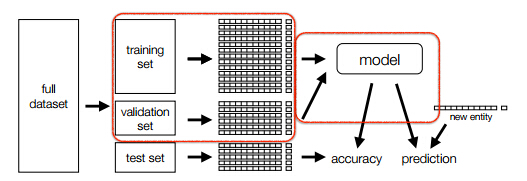
\includegraphics[height=4.5cm]{imagenes/crossValidation}
\caption{Cross Validation esquema}
\label{fig:exemplo}
\end{figure}

Este método será utilizado a en el desarrollo de este trabajo práctico. Más adelante explicaremos el porqué usarlo y los beneficios que trae.

